\documentclass[tikz]{standalone}

\usetikzlibrary{arrows.meta}
\tikzset{>=stealth}

\begin{document}
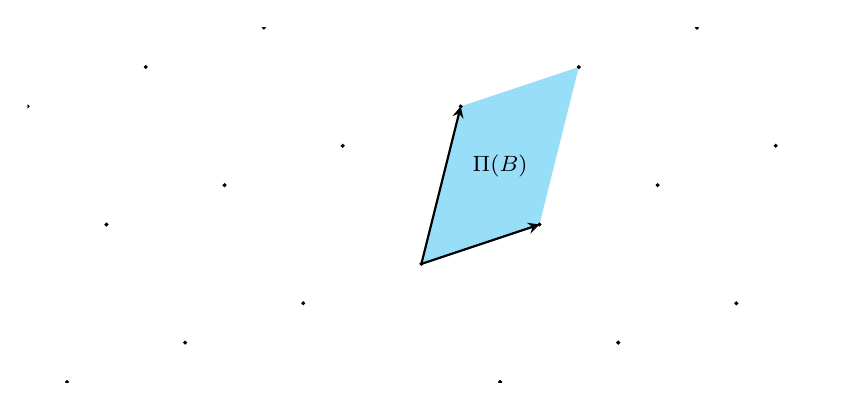
\begin{tikzpicture}[scale=0.5]
  \clip (-10, -3) rectangle (10, 6);
  \fill[color=cyan!40]
    (0, 0) -- (3, 1) -- ++(1, 4) -- (1, 4);
  \draw[->, thick] (0, 0) -- (3, 1);
  \draw[->, thick] (0, 0) -- (1, 4);
  \node at (2.0, 2.5) {\footnotesize$\Pi(B)$};

  \foreach \x in {-10,...,10}
  \foreach \y in {-10,...,10}
    \draw[fill] (3*\x + \y, \x + 4*\y) circle (1pt);
\end{tikzpicture}
\end{document}
